\documentclass[xcolor={svgnames}]{beamer}

\setbeameroption{hide notes} 

%\usetheme{NLP}
\usetheme{boxes}
\useoutertheme{infolines}

\usepackage{graphicx}
\usepackage{lmodern}
\usepackage{calc}

\usepackage{soul}

\usepackage{amsmath,amsthm,amssymb}   

\usepackage{listings}
\usepackage[style=authoryear,babel=hyphen]{biblatex}
\addbibresource{ref.bib}
\addbibresource{pliang.bib}

%\usepackage{algorithm,algorithmic}

\usepackage{tikz}
%\usepackage[debug,debugmarks]{scabby}
\usepackage[nodefinetheorems]{scabby}
\usepackage[beamer]{scabby-diag}

\usepackage[customcolors]{hf-tikz}

\usepackage{mathtools}

% Text
\newcommand{\todo}[1]{\hl{\textbf{TODO:} #1}}
\newcommand{\citationneeded} {\ensuremath{^{[\textrm{citation needed}]}}}


%Math Operators
%\DeclareMathOperator {\argmax} {argmax}
%\DeclareMathOperator {\argmin} {argmin}
\DeclareMathOperator {\sgn} {sgn}
\DeclareMathOperator {\trace} {tr}
\DeclareMathOperator{\E} {\mathbb{E}}
\DeclareMathOperator{\Var} {Var}
\DeclareMathOperator{\diag} {diag}
\DeclareMathOperator{\triu} {triu}
\DeclareMathOperator{\mult} {Multinomial}
\DeclareMathOperator{\normalt} {Normal}
\DeclareMathOperator{\cvec} {cvec}

\newcommand{\ud}{\, \mathrm{d}}
\newcommand{\diff}[1] {\frac{\partial}{\, \partial #1}}
\newcommand{\difff}[2] {\frac{\partial^2}{\, \partial #1\, \partial #2}}
\newcommand{\diffn}[2] {\frac{\partial^{#2}}{\, \partial {#1}^{#2}}}
\newcommand{\tuple}[1] {\langle #1 \rangle}
\newcommand{\innerprod}[2] {\langle #1, #2 \rangle}

% Constants/etc.
\renewcommand{\Re} {\mathbb{R}}
\newcommand{\Cm} {\mathbb{C}}
\newcommand{\Qm} {\mathbb{Q}}
\newcommand{\half} {\frac{1}{2}}

\newcommand{\inv}[1] {{#1}^{-1}}

\newcommand{\normal}[2] {\mathcal{N}(#1, #2)}
\newcommand{\mL} {\mathcal{L}}

\newcommand\eqdef{\ensuremath{\stackrel{\rm def}{=}}} % Equal by definition
\newcommand\refeqn[1]{(\ref{eqn:#1})}
\newcommand\sD{\ensuremath{\mathcal{D}}}
\newcommand\sM{\ensuremath{\mathcal{M}}}
\newcommand\refapp[1]{Appendix~\ref{sec:#1}}
\newcommand\refthm[1]{Theorem~\ref{thm:#1}}
\newcommand\sigmamin{\sigma_\text{\rm min}}
\newcommand\sigmamax{\sigma_\text{\rm max}}
\newcommand\op{{\text{\rm op}}}
\newcommand\BP{\ensuremath{\mathbb{P}}}
\newcommand\reflem[1]{Lemma~\ref{lem:#1}}

%% Tensor powers
\newcommand{\tp}[1] {^{\otimes #1}}

% Matrix Perturbation
\newcommand{\pinv}[1] {#1^{\dagger}}
\newcommand{\Ap} {\hat{A}}
\newcommand{\Bp} {\hat{B}}
\newcommand{\Up} {\hat{U}}
\newcommand{\Vp} {\hat{V}}
\newcommand{\Xp} {\hat{X}}
\newcommand{\Wp} {\hat{W}}
\newcommand{\cM} {\mathcal{M}}
\newcommand{\cMp} {\hat{\mathcal{M}}}
\newcommand{\Mp} {\hat{M}}
\newcommand{\Zp} {\hat{Z}}
\newcommand{\vp} {\hat{v}}
\newcommand{\lambdap} {\hat{\lambda}}
\newcommand{\sigmap} {\hat{\sigma}}
\newcommand{\mup} {\hat{\mu}}
\newcommand{\cnd}[1] {\kappa(#1)}
\newcommand{\aerr}[1] {\varepsilon_{#1}}
\newcommand{\rerr}[1] {\delta_{#1}}
\newcommand{\serr}[1] {\alpha_{#1}}
\newcommand{\berr}[1] {\beta_{#1}}
\newcommand{\gap}[1] {\Delta_{#1}}

% Keywords
\newcommand{\Pairs}{\mathrm{Pairs}}
\newcommand{\Triples}{\mathrm{Triples}}



\newcommand<>{\drawgen}[1]{%
  \uncover#2{
    \point{start-gen}{#1}
    \node[style=node] (h) at (start-gen) {};
    \node[left=0.1cm of h] {$h$};
    \node[style=node,fill=green!70,below=1cm of h] (x) {};
    \node[left=0.1cm of x] {$x$};
    \draw[-latex] (h) -- (x);
  }
}

\newcommand<>{\drawdisc}[1]{%
  \uncover#2{
    \point{start-disc}{#1}
    \node[style=node] (h) at (start-disc) {};
    \node[right=0.1cm of h] {$h$};

    \node[style=obsnode,left=0.3cm of h] (x) {};
    \node[left=0.1cm of x] {$x$};

    \node[style=obsnode,below=1cm of h] (y) {};
    \node[left=0.1cm of y] {$y$};
    \draw[-latex] (h) -- (y);
    \draw[-latex] (x) -- (y);
  }
}

\newcommand{\tensorfactorization}[1]{%
  \point{start-tf}{#1}
  \tikzcube{tensoring}{black,fill=white}{($(start-tf) + (0,0,0)$)}{1}{1}{1};
  \node at ($(tensoring) + (1.0cm,-0.3cm)$) {$=$};
  \tensorfiber{t1}{fill=blue!70}{($(tensoring) + (2.5cm,0.0cm)$)};
  \node at ($(t1) + (1.0cm,-0.3cm)$) {$+$};
  \tensorfiber{t2}{fill=green!70}{($(t1) + (2.5cm,0.0cm)$)};
  \node at ($(t2) + (1.0cm,-0.3cm)$) {$+ \dots + $};
  \tensorfiber{t3}{fill=red!70}{($(t2) + (3.0cm,0.0cm)$)};

  \draw [decorate,decoration={brace,amplitude=10pt,raise=4pt,mirror},yshift=0pt] 
    ($(t1) + (-1cm,-1cm)$) -- ($(t3) + (0.2cm,-1cm)$) node [below,black,midway,yshift=-0.6cm] {$k$};
}

\newcommand{\matrixfactorization}[1]{%
    \point{start-mf}{#1}
    \tikzrect{mat}{black,fill=white}{($(start-mf) + (0,0)$)}{1}{1};
    \node at ($(mat) + (1.0cm,-0.3cm)$) {$=$};
    \matfiber{t1}{fill=blue!70}{($(mat) + (2.5cm,0.0cm)$)};
    \node at ($(t1) + (1.0cm,-0.3cm)$) {$+$};
    \matfiber{t2}{fill=green!70}{($(t1) + (2.5cm,0.0cm)$)};
    \node at ($(t2) + (1.0cm,-0.3cm)$) {$+ \dots + $};
    \matfiber{t3}{fill=red!70}{($(t2) + (3.0cm,0.0cm)$)};
    \draw [decorate,decoration={brace,amplitude=10pt,raise=4pt,mirror},yshift=0pt] 
      ($(t1) + (-1cm,-1cm)$) -- ($(t3) + (0.2cm,-1cm)$) node [below,black,midway,yshift=-0.6cm] {$k$};
}

\newcommand{\llhood}[2]{%
  \begin{axis}[
      x=1cm,
      y=3cm,
      scale only axis,
      height=8cm,
      width=4cm,
      axis lines*=left,
      xtick=\empty,
      ytick=\empty,
      xlabel=$\theta$,
      ylabel=$-\log p_{\theta}(x)$
      ]
    \addplot[
        black,
        thick,
        smooth,
        ] file [% Provide data as a table
          ] {data/llhood.table}
     node[pos=0.27] (em1) {}
     node[pos=0.5] (spec) {}
     node[pos=0.61] (mle) {}
     node[pos=0.85] (em2) {}
     node[pos=0.9] (em2-start) {}
     ;

  \end{axis}
}

\newcommand{\mog}[2]{%
    \begin{axis}[
        xshift=#1,
        yshift=#2,
        scale only axis,
        height=3cm,
        width=3cm,
        axis lines*=left,
        xlabel=$x_1$,
        ylabel=$x_2$,
        xtick=\empty,
        ytick=\empty,
        mark options={scale=0.2,line width=0}
        ]
      \addplot+[
          smooth,
          only marks
          ] file [% Provide data as a table
            ] {data/mog-0.table};
      \addplot+[
          smooth,
          only marks
          ] file [% Provide data as a table
            ] {data/mog-1.table};
      \addplot+[
          smooth,
          only marks
          ] file [% Provide data as a table
            ] {data/mog-2.table}
       ;

    \end{axis}
}

\newcommand{\innerpdiag}[2]{%
  \node[scale=2.0] at ($#1 + (-1.3cm,-0.3cm)$) {$\langle$};
  \node at ($#1!0.5!#2 + (-0.3cm,-0.3cm) $) {$,$};
  \node[scale=2.0] at ($#2 + (0.8cm,-0.3cm)$) {$\rangle$};
}
\newcommand{\innerpdiagv}[2]{%
  \node[scale=2.0] at ($#1 + (-0.7cm,-0.45cm)$) {$\langle$};
  \node at ($#1!0.5!#2 + (-0.1cm,-0.45cm) $) {$,$};
  \node[scale=2.0] at ($#2 + (0.4cm,-0.45cm)$) {$\rangle$};
}
\newcommand{\innerpdiagm}[2]{%
  \node[scale=2.0] at ($#1 + (-1.3cm,-0.45cm)$) {$\langle$};
  \node at ($#1!0.5!#2 + (-0.5cm,-0.45cm) $) {$,$};
  \node[scale=2.0] at ($#2 + (0.4cm,-0.45cm)$) {$\rangle$};
}
\newcommand{\innerpdiagt}[2]{%
  \node[scale=2.0] at ($#1 + (-1.3cm,-0.3cm)$) {$\langle$};
  \node at ($#1!0.5!#2 + (-0.3cm,-0.3cm) $) {$,$};
  \node[scale=2.0] at ($#2 + (0.7cm,-0.3cm)$) {$\rangle$};
}

\newcommand{\regressionA}[1]{%
    \point{start-reg-a}{#1};
    \point{start-reg-a-A}{(start-reg-a)};
    \point{start-reg-a-B}{($(start-reg-a) + (1cm,0) $)};

    \tikzrect{A}{black,fill=yellow}{($(start-reg-a-A) + (0,0)$)}{0.3}{1};
    \tikzrect{B}{black,fill=blue!70}{($(start-reg-a-B) + (0,0)$)}{0.3}{1};
    \innerpdiagv{(start-reg-a-A)}{(start-reg-a-B)};
}

\newcommand{\regressionB}[1]{%
    \point{start-reg-b}{#1};
    \point{start-reg-b-A}{(start-reg-b)};
    \point{start-reg-b-B}{($(start-reg-b) + (1.5cm,0) $)};

    \tikzrect{A}{black,fill=yellow}{($(start-reg-b-A) + (0,0)$)}{1}{1};
    \tikzrect{B}{black,fill=blue!70}{($(start-reg-b-B) + (0,0)$)}{1}{1};
    \innerpdiagm{(start-reg-b-A)}{(start-reg-b-B)};
}

\newcommand{\regressionC}[1]{%
    \point{start-reg-c}{#1};
    \point{start-reg-c-A}{(start-reg-c)};
    \point{start-reg-c-B}{($(start-reg-c) + (1.8cm,0) $)};

    \tikzcube{A}{black,fill=yellow}{($(start-reg-c-A) + (0,0)$)}{1}{1}{1};
    \tikzcube{B}{black,fill=blue!70}{($(start-reg-c-B) + (0,0)$)}{1}{1}{1};
    \innerpdiagt{(start-reg-c-A)}{(start-reg-c-B)};
}


\newcommand{\mkmlrplot}[3]{%
\begin{tikzpicture}
\begin{axis}[ 
    xshift=#1, 
    yshift=#2, 
    height=5cm, width=5cm, 
    axis lines*=left, 
    xlabel=$x$, ylabel=$y$, 
    xtick=\empty, ytick=\empty, 
    mark options={scale=0.3,line width=0},
    xmin=-1.2, xmax=1.2,
    ]
  #3
\end{axis}
\end{tikzpicture}
}


\newcommand{\mlrfull}[2]{%
  \only<1>{%
    \mkmlrplot{#1}{#2}{%
       \addplot+[blue, line width=2pt, mark=none] {0.316 + -0.862*x};
       \addplot+[green,line width=2pt, mark=none] {-0.715 + -0.268*x};
       \addplot+[red,  line width=2pt, mark=none] {-1.076 + 0.595*x};
     }
  }
  \only<2>{%
    \mkmlrplot{#1}{#2}{%
       \addplot+[blue,                 mark=none] {0.316 + -0.862*x};
       \addplot+[green,                mark=none] {-0.715 + -0.268*x};
       \addplot+[red,  line width=2pt, mark=none] {-1.076 + 0.595*x};
     }
  }
  \only<3>{%
    \mkmlrplot{#1}{#2}{%
       \addplot+[blue,                 mark=none] {0.316 + -0.862*x};
       \addplot+[green,                mark=none] {-0.715 + -0.268*x};
       \addplot+[red,  line width=2pt, mark=none] {-1.076 + 0.595*x};
       \addplot[smooth, black, only marks] table {data/mlr-1.table};
     }
  }
  \only<4>{%
    \mkmlrplot{#1}{#2}{%
       \addplot+[blue, line width=2pt, mark=none] {0.316 + -0.862*x};
       \addplot+[green,                mark=none] {-0.715 + -0.268*x};
       \addplot+[red,                  mark=none] {-1.076 + 0.595*x};
       \addplot[smooth, black, only marks] table {data/mlr-1.table};
     }
  }
  \only<5>{%
    \mkmlrplot{#1}{#2}{%
       \addplot+[blue, line width=2pt, mark=none] {0.316 + -0.862*x};
       \addplot+[green,                mark=none] {-0.715 + -0.268*x};
       \addplot+[red,                  mark=none] {-1.076 + 0.595*x};
       \addplot[smooth, black, only marks] table {data/mlr-2.table};
     }
  }
  \only<6>{%
    \mkmlrplot{#1}{#2}{%
       \addplot[smooth, black, only marks] table {data/mlr.table};
       \addplot+[blue, line width=2pt, mark=none] {0.316 + -0.862*x};
       \addplot+[green,line width=2pt, mark=none] {-0.715 + -0.268*x};
       \addplot+[red,  line width=2pt, mark=none] {-1.076 + 0.595*x};
     }
  }
  \only<7>{%
    \mkmlrplot{#1}{#2}{%
       \addplot[smooth, black, only marks] table {data/mlr.table};
     }
  }
}

\newcommand{\mlrdata}[2]{%
    \mkmlrplot{#1}{#2}{%
     \addplot[smooth, black, only marks] table {data/mlr.table};
   }
}



% these will be used later in the title page
\title[Moments and Likelihoods]{Estimating Latent Variable Graphical Models with Moments and Likelihoods}
\author[Chaganty, Liang]{%
    Arun Tejasvi Chaganty\\
    Percy Liang
}
\institute{Stanford University}

\begin{document}

% "Beamer, do the following at the start of every section"
%\AtBeginSection[] 
\providecommand{\printoutline}
{%
\begin{frame}<beamer> 
\frametitle{Outline} % make a frame titled "Outline"
\todo{Make outline a diagram}
\tableofcontents[currentsection]  % show TOC and highlight current section
\end{frame}
}

\begin{frame}
  \titlepage
\end{frame}

\section{Introduction}

\begin{frame}
  \frametitle{Latent Variable Graphical Models}

  \splitcolumn{%
      \begin{itemize}
        \item Gaussian Mixture Models \tikzmark{gmm}
        \item Latent Dirichlet Allocation
        \item Hidden Markov Models \tikzmark{hmm}
        \item PCFGs
        \item \dots
      \end{itemize}
  }{%
  \begin{canvas}
    \point{mark}{(1cm,0)};
    \point{gmm}{($(mark) + (0,+0cm)$)};
    \point{hmm}{($(mark) + (0,-1cm)$)};

    \node[anchor=south west] (mog) at (gmm) {%
      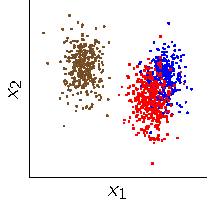
\includegraphics[width=0.45\textwidth,height=3cm,keepaspectratio]{figures/mog.pdf}
    };

    %\drawgen{($(gmm) + (0,0.0cm)$)};
    \drawhmm{(hmm)};
  \end{canvas}
  }

\end{frame}

\begin{frame}
  \frametitle{Parameter Estimation is Hard}

  \begin{tikzpicture}
    % x, y
    \llhood{0}{0};
    \node<2->[scale=0.3,circle,fill=black] at (mle) {};
    \node<2-> at ($(mle) + (0.6cm,0)$) {$\mathmb{\textrm{MLE}}$};
    \node<3->[scale=0.3,circle,fill=black] at (em1) {};
    \node<3-> at ($(em1) + (0.5cm,0)$) {$\mathmr{\textrm{EM}}$};
    \node<3->[scale=0.3,circle,fill=black] at (em2) {};
    \node<3-> at ($(em2) + (0.5cm,0)$) {$\mathmr{\textrm{EM}}$};

    \node<4->[scale=0.3,circle,fill=black] at (spec) {};
    \node<4-> at ($(spec) + (0.5cm,0.3cm)$) {$\mathmg{\textrm{MoM}}$};
   % \draw<4->[latex-latex,DarkGreen,line width=1pt] ($(mle) + (-0.8cm,0.8cm)$) -- node[above]{$\mathmg{\epsilon}$} ($(mle) + (+0.8cm,0.8cm)$);
  \end{tikzpicture}

  % Simple message: MLE is consistent but intractable, EM is efficient not but consistent. Can we get something in between.

  \begin{itemize}
    \item<1-> Log-likelihood function is non-convex.
    \item<2-> MLE is consistent but intractable.
    \item<3-> Local methods (EM, gradient descent, \dots) are tractable but inconsistent.
    \item<4-> {\em Method of moments} estimators can be consistent and
      computationally-efficient, but require more data. 
  \end{itemize}
\end{frame}

\begin{frame}
  \frametitle{Consistent estimation for general models}

  \begin{itemize}
    \item<+-> Several estimators based on the method of moments.
      \begin{itemize}
        \item {\bf Phylogenetic trees:} \cite{mossel2005learning}.
        \item {\bf Hidden Markov models:} \cite{hsu09spectral}
        \item {\bf Latent Dirichlet Allocation:} \cite{anandkumar12lda}
        \item {\bf Latent trees:} \cite{anandkumar11tree}
        \item {\bf PCFGs:} \cite{hsu12identifiability}
        \item {\bf Mixtures of linear regressors} \cite{chaganty13regression}
        \item {\bf \ldots}
      \end{itemize}
    \item<+-> These estimators are applicable only to a specific type of model. 
    \item<+-> In contrast, EM and gradient descent apply for almost any model.
    \item<+-> Note: some work in the observable operator framework does apply to a more general model class.
      \begin{itemize}
        \item {\bf Weighted automata:} \cite{balle12automata}.
        \item {\bf Junction trees:} \cite{song2011spectral}
        \item {\bf \ldots}
        \item \todo{Check that this list is representative}
      \end{itemize}
    \item<+-> {\bf How can we apply the method of moments to estimate {\em parameters efficiently} for a {\em general} model?}
  \end{itemize}
\end{frame}

\begin{frame}
  \frametitle{Setup}
  \splitcolumn{%
    \begin{itemize}
      \item Discrete models, $d$, $k$.
      \item Assume $d > k$.
      \item Parameters and marginals can be put into a matrix or tensor -> introduce notation.
      \item Assume infinite data.
      \item Highlight directed vs undirected - we focus on directed.
    \end{itemize}
  }{%
  }
  \end{frame}

\begin{frame}
  \frametitle{Background: Three-view Mixture Models}
  \cornertext<1->{}
  \splitcolumn{%
    \begin{definition}[Bottleneck]
      A hidden variable $h$ is a {\bf bottleneck} if there exist three
      observed variables ({\bf views}) $x_1, x_2, x_3$ that are
      {\em conditionally independent} given $h$.
    \end{definition}

    \begin{itemize}
      \item<2-> \cite{anandkumar12moments} provide an algorithm to estimate
        conditional moments $\Pr(x_i \given h)$ based on tensor eigendecomposition.
      \item<2-> In general, three views are necessary for identifiability
        (\cite{kruskal77three}).
    \end{itemize}
  }{%
    \begin{canvas}
        % The model
        \point{start}{(2cm,0cm)}; %{pic cs:gen} -| mark)};
        \drawgensquiggle<1->{($(start) + (1cm,1cm)$)};
        %\node[anchor=west] (diag1) at ($(start)$) {%
        %  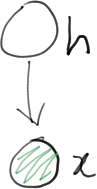
\includegraphics[width=0.45\textwidth,height=2cm,keepaspectratio]{figures/gen.png}
        %};
        %\node<1->[anchor=west] (diag) at ($(start) + (0cm,-1cm)$) {%
        %  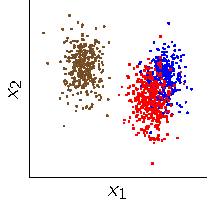
\includegraphics[width=0.45\textwidth,height=3cm,keepaspectratio]{figures/mog.pdf}
        %};
      \end{canvas}
  }
\end{frame}

\printoutline

\begin{frame}
  \frametitle{Example: a bridge, take I}
  \splitcolumn{%
    \begin{itemize}
      \item<1-> Each edge has a set of parameters.
      \item<2-> $h_1$ and $h_2$ are bottlenecks.
      \item<3-> We can learn $\Pr(x_1^a | h_1), \Pr(x_1^b | h_1), \cdots$.
      \item<5-> However, we can't learn $\Pr(h_2 | h_1)$ this way.
    \end{itemize}
  }{%
  \begin{canvas}
    \point{mark}{(3cm,0)};
    \drawbridge{(mark)};

  \begin{pgfonlayer}{background}
  \draw<2>[draw=black,fill=green!70,rounded corners,line width=1pt, dotted] 
                  ($(x1a.west) + (180:0.3cm)$) -- 
                  ($(h1.north) + (90:0.3cm)$) -- 
                  ($(x2a.east) + (0:0.3cm)$) -- 
                  ($(x2a.south) + (-90:0.3cm)$) -- 
                  ($(x1b.south) + (-90:0.3cm)$) -- 
                  ($(x1a.south) + (-90:0.3cm)$) -- 
                  cycle;
  \draw<2>[dashed,-latex] (h1) -- (x2a);
  \end{pgfonlayer}


   \uncover<3->{
   \draw[-latex,blue] (h1) -- (x1a);
   \draw[-latex,blue] (h1) -- (x1b);

   \draw[-latex,blue,dashed] (h1) -- (x2a);
   }

   %\uncover<4->{
   %\draw[-latex,blue,dashed] (h1) -- (x2b);
   %}

   \uncover<4->{
   \draw[-latex,blue] (h2) -- (x2a);
   \draw[-latex,blue] (h2) -- (x2b);
   %\draw[-latex,blue,dashed] (h2) -- (x1a);
   \draw[-latex,blue,dashed] (h2) -- (x1b);
   }

  \end{canvas}
  }
\end{frame}

\begin{frame}
  \frametitle{Example: a bridge, take II}
  \fontsize{8pt}{8.2pt}\selectfont
  \splitcolumn{%
    \begin{itemize}
      \item<1-> Observe the joint distribution,
        \todo{Use cartoon matrices}
        \begin{align*}
          \underbrace{\Pr(x_1^b, x_2^a)}_{M_{12}} &= \sum_{h_1, h_2} 
          \underbrace{\Pr(x_1^b \given h_1)}_{\mOpp{1}{1}}
          \underbrace{\Pr(x_2^a \given h_2)}_{\mOpp{2}{2}}
          \underbrace{\mathmb{\Pr(h_1, h_2)}}_{Z_{12}}.
        \end{align*}
      \item<2-> {\bf Observed moments} $\Pr(x_1^b, x_2^a)$ are {\em linear} in the {\bf hidden marginals} $\Pr(h_1, h_2)$.
        \begin{align*}
          M_{12} &= \mOpp{1}{1} Z_{12} \mOppt{2}{1}
        \end{align*}
      \item<3-> Solve for $\Pr(h_1, h_2)$ using pseudoinversion.
        \begin{align*}
          Z_{12} &= \mOppi{1}{1} M_{12} \mOppit{2}{1}
        \end{align*}
      \item<4-> $\Pr(h_2 \given h_1)$ can be recovered by normalization.
    \end{itemize}
  }{%
  \begin{canvas}
    \point{mark}{(3cm,0)};
    \point{start-bridge}{(mark)};

   \node[style=node, scale=0.8] (h1) at (start-bridge) {$h_1$};
   \node[style=node, scale=0.8, right= 1.0cm of h1] (h2) {$h_2$};
   \draw[-latex] (h1) -- (h2);

   %\point{V}{($(h4.north) + (0,0.1cm)$)};

% Observed nodes
   \node[style=obsnode, scale=0.6, below left=0.3cm of h1] (x1a) {$x_1^a$};
   \node[style=obsnode, scale=0.6, below=0.3cm of h1] (x1b) {$x_1^b$};
   \node[style=obsnode, scale=0.6, below=0.3cm of h2] (x2a) {$x_2^a$};
   \node[style=obsnode, scale=0.6, below right=0.3cm of h2] (x2b) {$x_2^b$};
   \draw[-latex,gray] (h1) -- (x1a);
   \draw[-latex,blue] (h1) -- (x1b);
   \draw[-latex,blue] (h2) -- (x2a);
   \draw[-latex,gray] (h2) -- (x2b);

  \end{canvas}
  }
\end{frame}

\printoutline

\section{Estimating Hidden Marginals}

\begin{frame}
  \frametitle{Exclusive Views}
  \splitcolumn{%
  \begin{definition}[Exclusive views]
    We say $h_i \in S \subseteq \bh$ has an {\bf exclusive view} $x_v$
      if
      \begin{enumerate}
        \item There exists some observed variable $x_{v}$ which is
          conditionally independent of the others $S \backslash \{ h_i \}$
          given $h_i$.
        \item The conditional moment matrix $\mOpp{v}{i} \eqdef
          \Pr(x_{v} \mid h_i)$ has full column rank $k$ and can be
          recovered.
        \item \todo{Exclusive views for a clique}
      \end{enumerate}
  \end{definition}
  }{%
  \begin{canvas}
    \point{mark}{(4cm,0)};
    \node at (mark) {%
      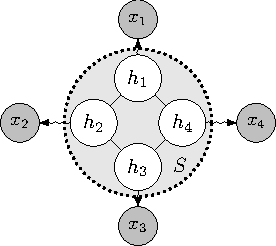
\includegraphics[width=0.5\textwidth,height=3cm,keepaspectratio]{figures/exclusive-views.pdf}
      };
  \end{canvas}
  }
\end{frame}

\begin{frame}
  \frametitle{Exclusive views give parameters}
  \splitcolumn{%
  \begin{itemize}
    \item Given {\em exclusive views}, $\Pr(x \given h)$,
      learning cliques is solving a linear equation!
        \todo{Use cartoon tensors}
      \begin{align*}
        \underbrace{\Pr(x_1, \ldots, x_m)}_{M} &=
        \sum_{h_1, \ldots, h_m}
        \underbrace{P(x_1 | h_1)}_{\mOpp{1}{1}} \cdots \\
        &\quad \hphantom{\sum_{h_1, \ldots, h_m}} \underbrace{\mathmb{P(h_1, \cdots, h_m)}}_{Z} \\
        \uncover<2->{
        M &= Z(\mOpp{1}{1}, \cdots, \mOpp{m}{m}) \\
        }
        \uncover<3->{
        Z &= M(\mOppi{1}{1}, \cdots, \mOppi{m}{m}).
        }
      \end{align*}
  \end{itemize}
  }{%
  \begin{canvas}
    \point{mark}{(4cm,0)};
    \node at (mark) {%
      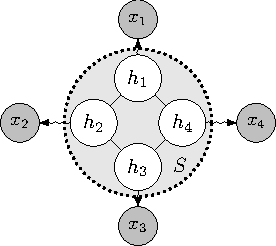
\includegraphics[width=0.5\textwidth,height=3cm,keepaspectratio]{figures/exclusive-views.pdf}
      };
  \end{canvas}
  }
\end{frame}

\begin{frame}
  \frametitle{Bottlenecked graphs}
  \splitcolumn{%
  \begin{itemize}
    \item<1-> When are we assured exclusive views?
  \end{itemize}
  \uncover<2->{
  \begin{definition}[Bottlenecked set]
    A set of hidden variables $S$ is said to be {\em bottlenecked} if
    each $h \in S$ is a bottleneck. 
  \end{definition}
  }
  \begin{itemize}
    \item<3-> {\bf Theorem:} A bottlenecked clique has exclusive views. \todo{Say show in paper.}
  \end{itemize}
  }{%
  \begin{canvas}
    \point{mark}{(4cm,0)};
    \node at (mark) {%
      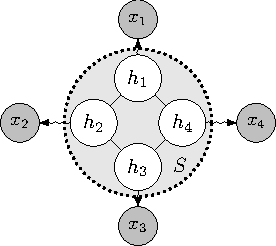
\includegraphics[width=0.5\textwidth,height=3cm,keepaspectratio]{figures/exclusive-views.pdf}
      };
  \end{canvas}
  }
\end{frame}

\printoutline

\begin{frame}
  \frametitle{Example}
  \begin{canvas}
    \point{mark}{(3cm,0)};
    \point{start-grid}{(mark)};
   \node[style=node, scale=0.8] (h1) at (start-grid) {$h_1$};
   \node[style=node, scale=0.8, below left= 0.5cm of h1] (h2) {$h_2$};
   \node[style=node, scale=0.8, below right= 0.5cm of h1] (h3) {$h_3$};
   \node[style=node, scale=0.8, below right= 0.5cm of h2] (h4) {$h_4$};

   \point{pi}{($(h1.north) + (0,0.1cm)$)};
   \draw[-latex] (h1) -- node[scale=0.7,above] (T1) {} (h2);
   \draw[-latex] (h1) -- node[scale=0.7,above] (T2) {} (h3);
   \draw[-latex] (h2) -- (h4);
   \draw[-latex] (h3) -- (h4);
   \point{V}{($(h4.north) + (0,0.1cm)$)};
  % Observed nodes
   \node[style=obsnode, scale=0.7, above left=0.3cm of h1] (x1a) {$x^a_1$};
   \node[style=obsnode, scale=0.7, above right=0.3cm of h1] (x1b) {$x^b_1$};
   \draw[-latex] (h1) -- (x1a);
   \draw[-latex] (h1) -- (x1b);

   \node[style=obsnode, scale=0.7, above left=0.3cm of h2] (x2a) {$x^a_2$};
   \node[style=obsnode, scale=0.7, below left=0.3cm of h2] (x2b) {$x^b_2$};
   \draw[-latex] (h2) -- node[scale=0.7,above] (O1) {} (x2a);
   \draw[-latex] (h2) -- node[scale=0.7,below] (O2) {} (x2b);

   \node[style=obsnode, scale=0.7, above right=0.3cm of h3] (x3a) {$x^a_3$};
   \node[style=obsnode, scale=0.7, below right=0.3cm of h3] (x3b) {$x^b_3$};
   \draw[-latex] (h3) -- (x3a);
   \draw[-latex] (h3) -- (x3b);
    
   \node[style=obsnode, scale=0.7, below left=0.3cm of  h4] (x4a) {$x^a_4$};
   \node[style=obsnode, scale=0.7, below right=0.3cm of h4] (x4b) {$x^b_4$};

   \draw[-latex] (h4) -- (x4a);
   \draw[-latex] (h4) -- (x4b);

   % Story - 
  \begin{pgfonlayer}{background}
  \draw<3>[draw=black,fill=green!70,rounded corners,line width=1pt, dotted] 
                  ($(x2a.north west) + (135:0.3cm)$) -- 
                  ($(x2b.south west) + (-135:0.3cm)$) -- 
                  ($(x4a.south east) + (-45:0.3cm)$) -- 
                  ($(h2.east) + (0:0.3cm)$) -- 
                  ($(x2a.north east) + (45:0.3cm)$) -- 
                  cycle;
  %  \draw<4>[draw=black,fill=green!70,rounded corners,line width=1pt, dotted] 
  %                  ($(x1a.north west) + (135:0.3cm)$) -- 
  %                  ($(x1a.north east) + (45:0.3cm)$) -- 
  %                  ($(h1.south east) + (-45:0.3cm)$) -- 
  %                  ($(h1.south west) + (-135:0.3cm)$) -- 
  %                  cycle;
  \draw<6>[draw=black,fill=green!70,rounded corners,line width=1pt, dotted] 
                  ($(x1b.north west) + (135:0.3cm)$) -- 
                  ($(x3a.north east) + (45:0.3cm)$) -- 
                  ($(h3.south east) + (-45:0.3cm)$) -- 
                  ($(h1.south west) + (-135:0.3cm)$) -- 
                  cycle;
  \draw<9>[draw=black,fill=green!70,rounded corners,line width=1pt, dotted] 
                  ($(h2.north west) + (135:0.3cm)$) -- 
                  ($(x2b.south west) + (-135:0.3cm)$) -- 
                  ($(x4a.south west) + (-135:0.3cm)$) -- 
                  ($(x4b.south east) + (-45:0.3cm)$) -- 
                  ($(x3b.north east) + (45:0.3cm)$) -- 
                  ($(h3.north east) + (45:0.3cm)$) -- 
                  cycle;
  \end{pgfonlayer}

  \draw<4>[blue,-latex, line width=1.3pt] (h2) -- (x2a);
  \draw<4>[blue,-latex, line width=1.3pt] (h2) -- (x2b);
  \draw<5->[blue,-latex] (h2) -- (x2a);
  \draw<5->[blue,-latex] (h2) -- (x2b);

  \draw<5>[blue,-latex,line width=1.3pt] (h1) -- (x1a);
  \draw<5>[blue,-latex,line width=1.3pt] (h1) -- (x1b);
  \draw<5>[blue,-latex,line width=1.3pt] (h3) -- (x3a);
  \draw<5>[blue,-latex,line width=1.3pt] (h3) -- (x3b);
  \draw<5>[blue,-latex,line width=1.3pt] (h4) -- (x4a);
  \draw<5>[blue,-latex,line width=1.3pt] (h4) -- (x4b);
  \draw<6->[blue,-latex] (h1) -- (x1a);
  \draw<6->[blue,-latex] (h1) -- (x1b);
  \draw<6->[blue,-latex] (h3) -- (x3a);
  \draw<6->[blue,-latex] (h3) -- (x3b);
  \draw<6->[blue,-latex] (h4) -- (x4a);
  \draw<6->[blue,-latex] (h4) -- (x4b);



  \draw<7>[blue,-latex, line width=1.3pt] (h1) -- (h3);
  \draw<8>[blue,-latex, line width=1.3pt] (h1) -- (h2);
  \draw<8->[blue,-latex] (h1) -- (h3);
  \draw<9->[blue,-latex] (h1) -- (h2);

  \draw<10>[blue,-latex, line width=1.3pt] (h2) -- (h4);
  \draw<10>[blue,-latex, line width=1.3pt] (h3) -- (h4);
  \draw<11->[blue,-latex] (h2) -- (h4);
  \draw<11->[blue,-latex] (h3) -- (h4);

  \end{canvas}
  
\end{frame}

\begin{frame}
  \frametitle{More Bottlenecked Examples}

  \cornertext<3->{\cite{halpern2013unsupervised}}
  \begin{canvas}
    \drawhmm<1->{(-4cm, 2cm)};
    \node at ($(start-hmm) + (0, 0.6cm)$) {Hidden Markov models};
    \drawtree<1->{(2cm, 2cm)};
    \node at ($(start-tree) + (0, 0.6cm)$) {Latent Tree models};
    \drawnoisyor<3->{(0cm, -2cm)};
    \node<3-> at ($(start-nor) + (0, 0.7cm)$) {Noisy Or (non-example)};

% \begin{pgfonlayer}{background}
% \draw<2->[rounded corners,line width=1pt, dotted, black] 
%                 ($(h2.north east) + (45:0.2cm)$) -- 
%                 ($(x3.north east) + (45:0.2cm)$) -- 
%                 ($(x3.south east) + (-45:0.2cm)$) -- 
%                 ($(x1.south west) + (-135:0.2cm)$) -- 
%                 ($(x1.north west) + (135:0.2cm)$) -- 
%                 ($(h2.north west) + (135:0.2cm)$) -- 
%                 cycle;
% \end{pgfonlayer}
% 
% \begin{pgfonlayer}{background}
% \draw<2>[rounded corners,line width=1pt, dotted, black] 
%                 ($(h4.north east) + (45:0.2cm)$) -- 
%                 ($(x4b.north east) + (45:0.2cm)$) -- 
%                 ($(x4b.south east) + (-45:0.2cm)$) -- 
%                 ($(x3b.south west) + (-135:0.2cm)$) -- 
%                 ($(x3b.north west) + (135:0.2cm)$) -- 
%                 ($(h4.north west) + (135:0.2cm)$) -- 
%                 cycle;
% \end{pgfonlayer}


  \end{canvas}

\end{frame}

% Efficiency 1: EM (+diagram).
\section{Combining moments with likelihood estimators}
\printoutline

\begin{frame}
  \frametitle{Convex marginal likelihoods}
  \splitcolumn{%
    \begin{itemize}
      \item<1-> The MLE is statistically
        most efficient, but usually non-convex. 
      \item<2-> If we fix the conditional moments, $-\log \Pr(x)$ is convex in $\theta$.
      \item<3-> No closed form solution, but a local method like EM is
        guaranteed to converge to the global optimum.
    \end{itemize}
  }{%
    \begin{canvas}
      \point{stuff}{(2cm,2.5cm)};
      \drawbridge<1->{(stuff)};
      \node[scale=0.8] at ($(start-bridge) - (-1,2.5cm)$) {\obj{
      \begin{align*}
        \log \Pr(\bx) &= \log \sum_{h_1,h_2} 
        \robustaltm<1>{
        \mathmb{\Pr(\bx_1 | h_1) \Pr(\bx_2 | h_2)}
        }{
        \underbrace{\Pr(\bx_1 | h_1) \Pr(\bx_2 | h_2)}_{\text{known}} 
        }
        \mathmb{\Pr(h_1, h_2)}
      \end{align*}
      }};
      \node<2->[scale=0.8,anchor=north] at ($(start-bridge) - (-1cm,3.0cm)$) {
      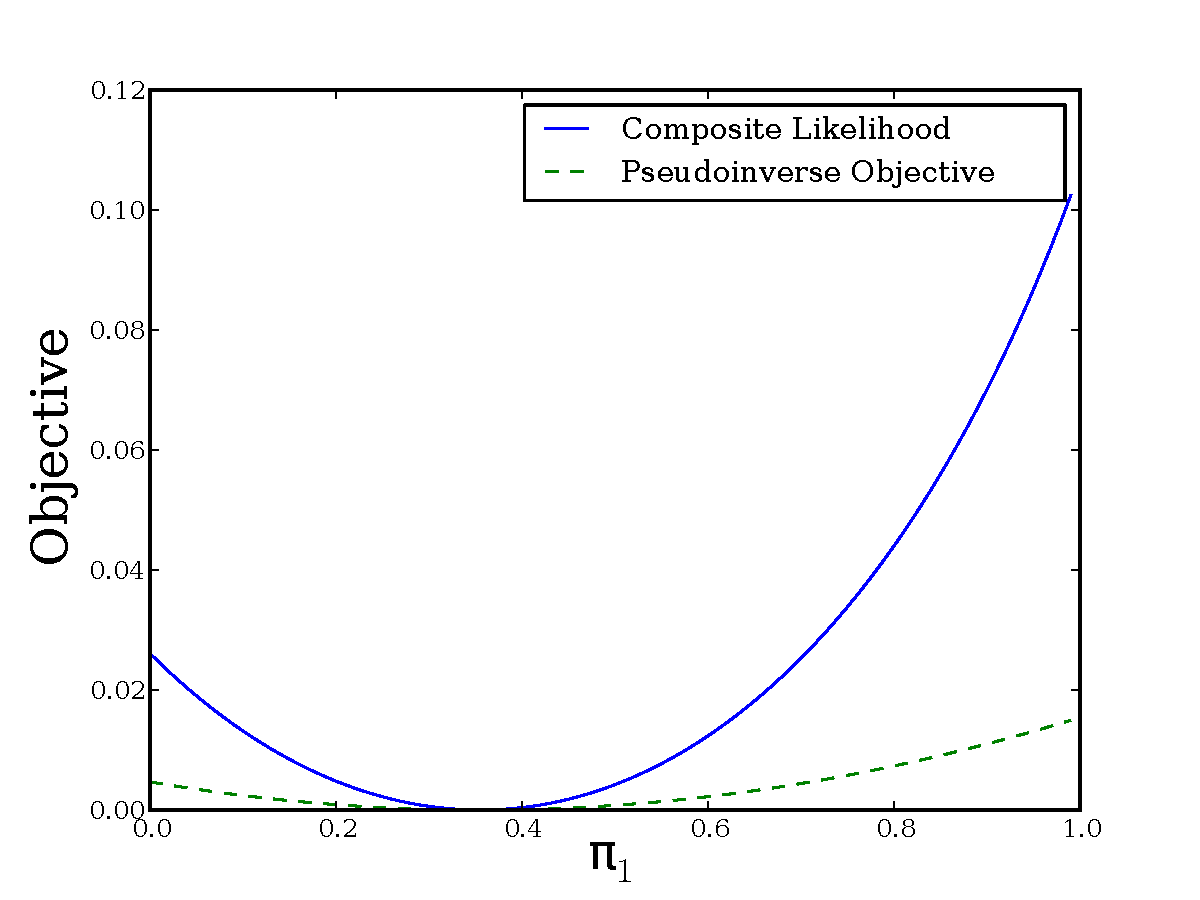
\includegraphics[width=\textwidth,height=6cm,keepaspectratio]{figures/piecewise-objective.pdf}
      };
    \end{canvas}
  }
\end{frame}

\begin{frame}
  \frametitle{Composite likelihoods}
  \splitcolumn{%
    \begin{itemize}
      \item<1-> In general, the full likelihood is still non-convex. \todo{Specify which x}.
      \item<2-> Consider {\em composite likelihood} on a subset of observed variables.
      \item<4-> Can be shown that estimation with composite likelihoods is consistent (\cite{lindsay88composite}).
      \item<4-> Asymptotically, the composite likelihood estimator is more efficient.
    \end{itemize}
  }{%
    \begin{canvas}
      \point{stuff}{(2cm,2.5cm)};
      \drawhmm<1->{(stuff)};
      \node<1-2>[scale=0.8] at ($(start-hmm) - (-1,2.5cm)$) {\obj{
      \begin{align*}
        \log \Pr(\bx) &= \log \sum_{h_1,h_2,h_3} \underbrace{\Pr(\bx_1 \given h_1) \Pr(\bx_2 \given h_2)  \robustaltm<1>{\Pr(\bx_3 \given h_3)}{\mathmr{\Pr(\bx_3 \given h_3)}}}_{\text{known}} \\ 
        &\quad \hphantom{\log \sum_{h_1,h_2,h_3} } 
        \robustaltm<1>{\mathmb{\Pr(h_3 \given h_2)}}{\mathmr{\Pr(h_3 \given h_2)}} \mathmb{\Pr(h_1, h_2)}
      \end{align*}
      }};

      \begin{pgfonlayer}{background}
      \draw<2->[draw=black,fill=green!70,rounded corners,line width=1pt, dotted] 
                      ($(h1.west) + (180:0.3cm)$) -- 
                      ($(h1.north) + (90:0.3cm)$) -- 
                      ($(h2.north) + (90:0.3cm)$) -- 
                      ($(h2.east) + (0:0.3cm)$) -- 
                      ($(x2.east) + (0:0.3cm)$) -- 
                      ($(x2.south) + (-90:0.3cm)$) -- 
                      ($(x1.south) + (-90:0.3cm)$) -- 
                      ($(x1.west) + (180:0.3cm)$) -- 
                      cycle;
      \end{pgfonlayer}

      \node<3->[scale=0.8] at ($(start-hmm) - (-1,2.5cm)$) {\obj{
      \begin{align*}
        \log \Pr(\bx) &= \log \sum_{h_1,h_2} \underbrace{\Pr(\bx_1 \given h_1) \Pr(\bx_2 \given h_2)}_{\text{known}} \\ 
        &\quad \hphantom{\log \sum_{h_1,h_2} } \mathmb{\Pr(h_1, h_2)}
      \end{align*}
      }};
      \begin{pgfonlayer}{background}
      \node<4->[scale=0.8,anchor=north] at ($(start-bridge) - (-1cm,3.3cm)$) {
      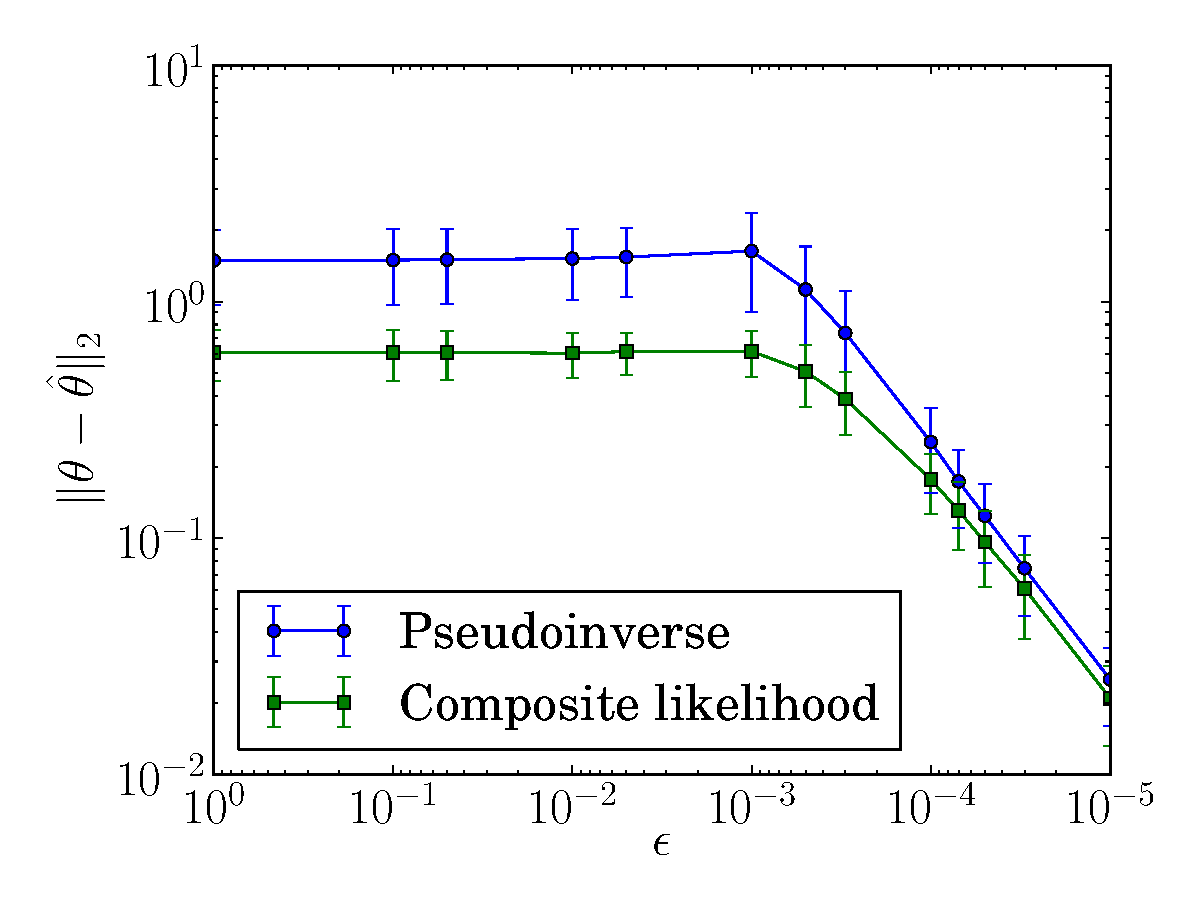
\includegraphics[width=\textwidth,height=6cm,keepaspectratio]{figures/asymp-k2d5.pdf}
      };
      \end{pgfonlayer}
    \end{canvas}
  }
\end{frame}


\section{Recovering parameters}
\printoutline

\begin{frame}
  \frametitle{Recovering parameters in directed models}
  \splitcolumn{%
  \begin{itemize}
    \item Conditional probability tables are the default
      parameterization for a directed model. 
    \item Can be recovered by normalization:
      \begin{align*}
        \Pr(h_2 \given h_1) &= \frac{\Pr(h_1, h_2)}{\sum_{h_2} \Pr(h_1, h_2)}.
        \end{align*}
  \end{itemize}
  }{%
    \begin{canvas}
      \point{stuff}{(2cm,0cm)};
      \drawbridge<1->{(stuff)};
      \node[scale = 0.5, anchor=south] at (h1h2) {
        \begin{tabular}{r | l l}
          \diaghead{aaaaaa}{$h_2$}{$h_1$} &
          \thead{$0$} & \thead{$1$} \\ \hline 
          $0$ & \quad & \quad \\ 
          $1$ & \quad & \quad 
        \end{tabular}
      };
    \end{canvas}
  }
\end{frame}

\begin{frame}
  \frametitle{Recovering parameters in undirected log-linear models}
  \fontsize{8pt}{8.2pt}\selectfont

  \splitcolumn{%
    \begin{itemize}
      \item<1-> Assume a log-linear parameterization, \todo{use sum over cliques - talk through}.
        \begin{align*}
        p_\theta(\bx, \bh) &= \exp\left( \theta^\top \phi(\bx,\bh) - A(\theta) \right).
        \end{align*}
      \item<2-> The {\em unsupervised} negative log-likelihood is non-convex,
          \begin{align*}
            \sL_\text{unsup}(\theta) \eqdef \E_{\bx \sim \sD}[- \log \mathmr{ \sum_{\bh \in \sH} p_\theta(\bx,\bh)} ].
          \end{align*}
      \item<3-> However, the {\em supervised} negative log-likelihood is convex,
          \begin{align*}
          \sL_\text{sup}(\theta) &\eqdef \E_{(\bx,\bh) \sim \sD_\text{sup}}\left[- \log p_\theta(\bx,\bh) \right] \\
          &= -\mathmb{\theta^\top} \left(\sum_{\sC \in \sG} \E_{(\bx,\bh) \sim \sD_\text{sup}}[\phi(\bx_\sC,\bh_\sC)]\right) + \mathmb{A(\theta)}.
          \end{align*}
    \end{itemize}
  }{%
    \begin{canvas}
      \point{stuff}{(2cm,0cm)};
      \drawubridge<1->{(stuff)};
      \node[scale = 1.0, anchor=south] at (h1h2) {$\theta$};
    \end{canvas}
  }
\end{frame}

\begin{frame}
  \frametitle{Recovering parameters in undirected log-linear models}
  \fontsize{8pt}{8.2pt}\selectfont

  \splitcolumn{%
    \begin{itemize}
      \item<1-> Recall, the marginals can typically estimated from
        supervised data. 
          \begin{align*}
          \label{eqn:logLinearSupervised}
          \sL_\text{sup}(\theta) &= -\mathmb{\theta^\top} \mathmg{\underbrace{\left(\sum_{\sC \in \sG} \E_{(\bx,\bh) \sim \sD_\text{sup}}[\phi(\bx_\sC,\bh_\sC)]\right)}_{\mu_\sC}} + \mathmb{A(\theta)}.
          \end{align*}
        \item<2-> However, the marginals can also be {\em consistently}
          estimated by moments!
        \begin{align*}
          \mu_\sC &= \sum_{\bx_\sC, \bh_\sC} \underbrace{\mathmg{\Pr(\bx_\sC \given \bh_\sC)}}_{\textmg{cond. moments}} 
          \underbrace{\mathmb{\Pr(\bh_\sC)}}_{\textmb{hidden marginals}} \phi(\bx_\sC,\bh_\sC).
        \end{align*}
    \end{itemize}
  }{%
    \begin{canvas}
      \point{stuff}{(2cm,0cm)};
      \drawubridge<1->{($(stuff) + (0,0cm)$)};
      \node[scale = 1.0, anchor=south] at (h1h2) {$\theta$};
    \end{canvas}
  }
\end{frame}

\begin{frame}
  \frametitle{Optimizing pseudolikelihood}
  \fontsize{8pt}{8.2pt}\selectfont

  \splitcolumn{%
    \begin{itemize}
        \item<1-> Estimating marginals $\mu_\sC$ is independent of treewidth, but 
          computing the normalization constant is: \todo{convex but not easy}
          \begin{align*}
            A(\theta) &\eqdef \log \sum_{\bx, \bh} \exp\left(\theta^\top \phi(\bx, \bh) \right).
          \end{align*}
        \item<2-> We can use pseudolikelihood (\cite{besag75pseudo}) to consistently estimate
          distributions over local neighborhoods. 
          \begin{align*}
            A_{\text{pseudo}}(\theta; \sN(a)) &\eqdef \log \sum_{a} \exp\left(\theta^\top \phi(\bx_\sN, \bh_\sN) \right).
          \end{align*}
        \item<3-> Clique marginals not sufficient statistics, but we can still estimate them.
    \end{itemize}
  }{%
    \begin{canvas}
      \point{stuff}{(2cm,0cm)};
      \node at ($(stuff) + (1cm,0cm)$) {
      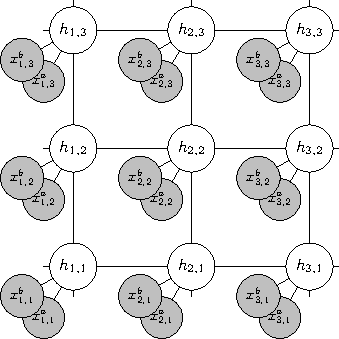
\includegraphics[width=0.45\textwidth,height=3cm,keepaspectratio]{figures/mrf.pdf}
      };
    \end{canvas}
  }
\end{frame}

\section{Conclusions}

\begin{frame}
  \frametitle{Conclusions}
  %\begin{itemize}
  %    \item Uniformly bottlenecked models
  %    \item Scales with the size of each clique, not the tree-width
  %    \item Solving bottlenecks breaks problem into convex pieces; can be solved more accurately
  %    \item The marginals make the log-linear recovery problem convex.
  %\end{itemize}
  \splitcolumn{%
    \begin{itemize}
     % \item {\em Before our work}
     % \begin{itemize}
     %   \item Gaussian Mixture Models \tikzmark{gmm}
     %   \item Hidden Markov Models 
     %   \item Latent Dirichlet Allocation
     % \end{itemize}
     \item \todo{Use outline slide}.
     \item \todo{Show the venn diagram on progress on generality.}.
     \item<1-> An algorithm for any (non-degenerate) {\bf bottlenecked discrete graphical models}. \tikzmark{grid}
    \item<2-> Efficiently learns models with {\bf high-treewidth}.
    \item<3-> Combine moment estimators with composite
      likelihood estimators.
    \item<4-> Extends to {\bf log-linear models}.
      \begin{itemize}
        \item Allows for easy regularization, missing data, etc.
      \end{itemize}
    \end{itemize}
  }{%
  \begin{canvas}
    \point{mark}{(4cm,0)};
    %\point{gmm}{({pic cs:gmm} -| mark)};
    %\point{grid}{({pic cs:grid} -| mark)};
    %\point{gmm}{($(mark) + (0,3cm)$)};
    \point{grid}{($(mark) + (0,1cm)$)};

%    \node[anchor=south west] (mog) at (gmm) {%
%      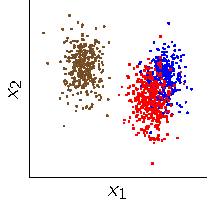
\includegraphics[width=0.45\textwidth,height=3cm,keepaspectratio]{figures/mog.pdf}
%    };

    %\drawgen{($(gmm) + (0,0.0cm)$)};
    \drawgrid{(grid)};
  \end{canvas}
  }


%  \cornertext<1->{\cite{AnandkumarGeHsu2012}}
%
%  \begin{canvas}
%    % Tasks.
%
%    \node<1->[anchor=west] (diag) at (-3cm, 1cm) {%
%      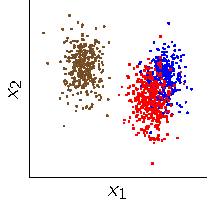
\includegraphics[width=0.45\textwidth,height=3cm,keepaspectratio]{figures/mog.pdf}
%    };
%    %\drawgen{(-3cm,1cm)}
%    \node[below=0.6cm of diag.south] {Before};
%
%    % Highlight
%    \draw<2>[scale=0.8,fill=green,opacity=0.4,dashed] (1cm,2.5cm) rectangle (6.5cm,-2.5cm);
%      \drawgrid{(3cm,1cm)}
%      \node[below=0.1cm of h4.south] {After};
%  \end{canvas}

\end{frame}



\begin{frame}
  \frametitle{}
    Thank you!
\end{frame}

\end{document}

